% WICHTIGE INFO:
% für die grundsätzlichen Daten der Titelpage bitte 
% die Definitionen in der0 phdthesis.sty Datei pflegen!
% WICHTIGE INFO ENDE


\documentclass[a4paper,11pt]{book} %draft%

\usepackage{amsmath,amsfonts,amssymb,bbm}	
\usepackage{graphicx}						% Einbinden von Bildern
\usepackage{phdthesis}						% Styledatei
\usepackage[utf8]{inputenc}					% Umlaute
\usepackage{epstopdf}						% einbinden von .eps Dateien in pdflatex, erfordert ghostscript
\usepackage{psboxit}
\usepackage[ngerman]{babel}					% Formatierungen in deutscher Sprache z.B. Datum

\usepackage{blindtext}						% Lorem Ipsum
\usepackage[colorinlistoftodos]{todonotes} 	%\todo, \missingfigure und \listoftodos (siehe unten für eigene Definitionen)


\usepackage[sort]{natbib}					% Zitationstyle
\usepackage{bibunits}						% Einbinden mehrerer Literaturverzeichnisse


\usepackage{nicefrac}						% schönere Darstellung von Brüchen
\usepackage{subcaption}						% Bildunterschriften mehrerer Subfigures 
\usepackage{multirow}						% Tabellen mit Zeilen und Spaltenverbunden
\usepackage[]{caption}						% Bildunterschriften bei mehreren Teilgrafiken in einer Figure
\usepackage{catoptions}						


% EIGENE (Christoph Dollase)
\usepackage{csquotes}
\usepackage{tcolorbox}
\newtcolorbox
[auto counter,number within=section]{bsp}[2][]{
	colback=black!5!black,colframe=black!40!white,fonttitle=\bfseries,
	title=Bsp.~
	\thetcbcounter
	: #2,#1}
%\newtcolorbox[auto counter,number within=chapter]{bsp}[1][]{
%	fonttitle=\scshape,
%	title={Bsp. \thetcbcounter},
%	#1}

% Todo Notationen
% -----------------------------------------------------------
\newcommand{\newtodo}[1]{\todo[inline, color=yellow!90]{#1}}
\newcommand{\wichtig}[1]{\todo[inline, color=red!65]{#1}}  
\newcommand{\reread}[1]{\todo[color=green!90]{#1}}
\newcommand{\change}[1]{\todo[color=blue!40]{#1}}
\newcommand{\info}[1]{\todo[color=white, bordercolor=black]{#1}}


% ENDE EIGENE

% Schriftart und Textformatierungen
% -----------------------------------------------------------
\usepackage{fourier}        
\DeclareMathAlphabet{\mathcal}{OMS}{cmsy}{m}{n}
\usepackage{scalefnt}
\usepackage[scaled=0.875]{helvet} % ss
\renewcommand{\ttdefault}{lmtt} %tt
\usepackage{microtype}						% Verbesserungen im Texfluss
\setlength{\emergencystretch}{1em}

\DeclareFontFamily{U}{rcjhbltx}{}
\DeclareFontShape{U}{rcjhbltx}{m}{n}{<->rcjhbltx}{}
\DeclareSymbolFont{hebrewletters}{U}{rcjhbltx}{m}{n}
\DeclareMathSymbol{\ayin}{\mathord}{hebrewletters}{96}
\DeclareMathSymbol{\beth}{\mathord}{hebrewletters}{98}\let\bet\beth


% Literaturverzeichnis und Inhaltslisten (Bilder, Tabellen, Algorithmen)
% ----------------------------------------------------------
\usepackage{tocloft}						% Beeinflussen des Literaturverzeichnisses und anderer Inhaltslisten


% Tabellenformatierung
% ----------------------------------------------------------
\usepackage{pgfplotstable}
\usepackage{booktabs}
\usepackage{slashbox}

% EIGENE Tabellen anpassung
\usepackage{tabularx}
\newcolumntype{L}[1]{>{\raggedright\arraybackslash}p{#1}} % linksbündig mit Breitenangabe
\newcolumntype{C}[1]{>{\centering\arraybackslash}p{#1}} % zentriert mit Breitenangabe
\newcolumntype{R}[1]{>{\raggedleft\arraybackslash}p{#1}} % rechtsbündig mit Breitenangabe
% ENDE

% Schusterjungen und Hurenkinder bestrafen
% -----------------------------------------------------------
\clubpenalty = 10000 
\widowpenalty = 10000 
\displaywidowpenalty = 10000


% Darstellungen von Graphen
% -----------------------------------------------------------
\usepackage{tikz}

%\usepackage[pdfborder	={0 0 0}]{hyperref}
\usepackage[hidelinks]{hyperref}


\makeatletter
\pgfdeclarelayer{background}
\pgfdeclarelayer{foreground}
\pgfsetlayers{background,main,foreground}



% Algorithmen und Pseudocode
% -----------------------------------------------------------
\usepackage{algorithmic}
\usepackage{algorithm} 
\renewcommand{\listalgorithmname}{Algorithmenverzeichnis}
\floatname{algorithm}{Algorithmus} 
\renewcommand{\algorithmicrequire}{\textbf{Eingabe:}} 
\renewcommand{\algorithmicensure}{\textbf{Ausgabe:}} 
\renewcommand{\algorithmicreturn}{\textbf{Rückgabe:}} 
%\renewcommand{\algorithmifloatname}{\textbf{Algorithmus}} 
\renewcommand{\algorithmicwhile}{\textbf{So lange}} 
\renewcommand{\algorithmicforall}{\textbf{Für alle}} 
\renewcommand{\algorithmicif}{\textbf{Wenn}} 
\renewcommand{\algorithmicthen}{\textbf{dann}} 
\renewcommand{\algorithmicendif}{\textbf{Wenn Ende}} 
\renewcommand{\algorithmicdo}{\textbf{führe aus}} 
\renewcommand{\algorithmicendfor}{\textbf{Für alle Ende}} 
\renewcommand{\algorithmicendwhile}{\textbf{So lange Ende}} 


\parskip1ex
\parindent0em


% Notationen
% -----------------------------------------------------------
\DeclareMathOperator{\lift}{lift}
\newcommand{\indep}{\rotatebox[origin=c]{90}{$\models$}}


% Zahlenbereiche
% -----------------------------------------------------------
\newcommand{\Integer}[0]{\mathrm{Z\hspace{-0.4em}Z}}
\newcommand{\Natural}[0]{\mathrm{I\hspace{-0.8mm}N}}
\newcommand{\Real}[0]{\mathrm{I\hspace{-0.8mm}R}}


% "\headheight is too small"-Warnung loswerden
\setlength{\headheight}{15pt}


% \tocless verhindert die Aufnahme ins IHV
% (behaelt aber Nummerierung bei)
%-----------------------------------------------------------------------------
\newcommand{\nocontentsline}[3]{}
\newcommand{\tocless}[2]{\bgroup\let\addcontentsline=\nocontentsline#1{#2}\egroup}



% Umgebungsdefinitionen
%----------------------------------------------------------
\newtheorem{theorem}{Theorem}
%\newtheorem{acknowledgement}[theorem]{Acknowledgement}
%\newtheorem{algorithm}[theorem]{Algorithm}
%\newtheorem{axiom}[theorem]{Axiom}
%\newtheorem{case}[theorem]{Case}
%\newtheorem{claim}[theorem]{Claim}
%\newtheorem{conclusion}[theorem]{Conclusion}
%\newtheorem{condition}[theorem]{Condition}
%\newtheorem{conjecture}[theorem]{Conjecture}
%\newtheorem{corollary}[theorem]{Corollary}
%\newtheorem{criterion}[theorem]{Criterion}
\newtheorem{definition}[theorem]{Definition}
%\newtheorem{example}[theorem]{Example}
%\newtheorem{exercise}[theorem]{Exercise}
%\newtheorem{lemma}[theorem]{Lemma}
%\newtheorem{notation}[theorem]{Notation}
%\newtheorem{problem}[theorem]{Problem}
%\newtheorem{proposition}[theorem]{Proposition}
%\newtheorem{remark}[theorem]{Remark}
%\newtheorem{solution}[theorem]{Solution}
%\newtheorem{summary}[theorem]{Summary}
%\newenvironment{proof}[1][Proof]{\textbf{#1.} }{\ \rule{0.5em}{0.5em}}


% Farbdefinitionen
%-----------------------------------------------------------------------------
\definecolor{blue}{RGB}{102,102,255}
\definecolor{green}{RGB}{152,223,138}
\definecolor{violet}{RGB}{148,103,189}
\definecolor{pablue}{RGB}{0,77,128}
\definecolor{palightlue}{RGB}{0,143,213}
\definecolor{pagreen}{RGB}{153,204,51}
\definecolor{paorange}{RGB}{255,153,51}



% Sorgt dafuer, dass die mit dem Package footmisc einzugslosen Fusznotennummern
% nicht auszerhalb des linken Randes sind....
% -----------------------------------------------------------
\makeatletter
\newlength{\myFootnoteWidth}
\newlength{\myFootnoteLabel}
\setlength{\myFootnoteLabel}{0.7em}%  <-- can be changed to any valid value
\renewcommand{\@makefntext}[1]{%
  \setlength{\myFootnoteWidth}{\columnwidth}%
  \addtolength{\myFootnoteWidth}{-\myFootnoteLabel}%
  \noindent\makebox[\myFootnoteLabel][r]{\@makefnmark\ }%
  \parbox[t]{\myFootnoteWidth}{#1}%
}

% capitalized reference
\def\Autoref#1{%
	\begingroup
	\edef\reserved@a{\cpttrimspaces{#1}}%
	\ifcsndefTF{r@#1}{%
		\xaftercsname{\expandafter\testreftype\@fourthoffive}
		{r@\reserved@a}.\\{#1}%
	}{%
	\ref{#1}%
}%
\endgroup
}
\def\testreftype#1.#2\\#3{%
	\ifcsndefTF{#1autorefname}{%
		\def\reserved@a##1##2\@nil{%
			\uppercase{\def\ref@name{##1}}%
			\csn@edef{#1autorefname}{\ref@name##2}%
			\autoref{#3}%
		}%
		\reserved@a#1\@nil
	}{%
	\autoref{#3}%
}%
}

% Definition von Mehrfachreferenzen
\newcommand\multref[1]{\@first@ref#1,@}
\def\@throw@dot#1.#2@{#1}% discard everything after the dot
\def\@set@refname#1{%    % set \@refname to autoefname+s using \getrefbykeydefault
	\edef\@tmp{\getrefbykeydefault{#1}{anchor}{}}%
	\def\@refname{\@nameuse{\expandafter\@throw@dot\@tmp.@autorefname}s}%
}
\def\@first@ref#1,#2{%
	\ifx#2@\autoref{#1}\let\@nextref\@gobble% only one ref, revert to normal \autoref
	\else%
	\@set@refname{#1}%  set \@refname to autoref name
	\@refname~\ref{#1}% add autoefname and first reference
	\let\@nextref\@next@ref% push processing to \@next@ref
	\fi%
	\@nextref#2%
}
\def\@next@ref#1,#2{%
	\ifx#2@ and~\ref{#1}\let\@nextref\@gobble% at end: print and+\ref and stop
	\else, \ref{#1}% print  ,+\ref and continue
	\fi%
	\@nextref#2%
}

% roman numbers
\newcommand*{\rom}[1]{\expandafter\@slowromancap\romannumeral #1@}
\makeatother


% Kürzel für Fließtexte
% -----------------------------------------------------------
\newcommand{\etc}{etc.\xspace}

% Befehle für Matheumgebungt
% -----------------------------------------------------------
\DeclareMathOperator*{\argmin}{arg\,min}

% Befehle für Matheumgebung und Fließtext
% -----------------------------------------------------------
\newcommand{\epsneighborhood}{\ensuremath{\epsilon}-neigh\-bor\-hood\xspace}

% Silbentrennung (speziell für Namen relevant)
% -----------------------------------------------------------
\hyphenation{Ag-ra-wal}
 


\makeindex
\cftpagenumbersoff{chapter}
\begin{document}

% =============================================================================
	\frontmatter

	%\input{chapter/front}
	
\begin{titlepage}
  \thispagestyle{titlepage}
  \begin{center}
  {\LARGE \myuniversity}\\[10mm]
  \begin{figure*}[h]
   \hbox{}\hfill
   \begin{minipage}[t]{9cm}
			 \centering
			 % LOGO DEINER UNI/FAKULTÄT HIER EINFÜGEN
			 
\includegraphics[width=7cm]{logos/OVGU_SIGN_druck.eps}
   \end{minipage}
   \hfill\hbox{}
  \end{figure*}
  {\large \myschool\\ \mydepartment}\\[10mm]
  {\LARGE \kindOfThesis}\\[5mm]
		%{\large\bf \titleOfThesis}\\[10mm]
		{\Large\bf \titleOfThesis}\\[10mm]
  {\small Author:}\\[1mm]
  {\large \myfirstname~\mylastname}\\[5mm]
  {\small \today}\\[5mm]
   
  \vspace{3cm}
  %BETREUER HIER
  \begin{tabular}{c}
  	\multicolumn{1}{c}{\small Betreuer:} \\[1mm]
  	{\small Prof. Dr.}  \\
  	{\large Attila Hunnenking} \\[2mm]
  	{\small \myschool}  \\
  	{\small \myuni}	\\
  	{\small \myunistreet} \\
  	{\small \myunizipcity}
  \end{tabular} \\[5mm]

 
\renewcommand{\arraystretch}{1}
  \end{center}
\end{titlepage}

\thispagestyle{empty}
\vspace*{\fill}
\cleardoublepage

\thispagestyle{empty}
\vspace*{\fill}
\begin{minipage}{.95\textwidth}
\textbf{\mylastname,~\myfirstname:}\\
\emph{\titleOfThesis}\\
\kindOfThesis, \myuni \\
\myplace, \myyear.
\end{minipage}

\clearpage

% =============================================================================

%%%%%%%%%%%%%%%%%%%%%%%%%%%%%%%%%%%%%%%%%%%%%%%%%%%%%%%%%%%%%%%%%%%%%%%%%%%%%
%%% Inhaltsverzeichnis
%%%%%%%%%%%%%%%%%%%%%%%%%%%%%%%%%%%%%%%%%%%%%%%%%%%%%%%%%%%%%%%%%%%%%%%%%%%%%
%INFO tocdepths gibt Detailgrad des Inhaltsverzeichnus, also ob nur Sections oder sogar SubSubSections {3} angezeigt werden sollen
\setcounter{tocdepth}{2} 
\tableofcontents

%\addcontentsline{toc}{chapter}{Abbildungsverzeichnis} %ist im appendix
%\listoffigures

%\addcontentsline{toc}{chapter}{Tabellenverzeichnis} %ist im appendix
%\listoftables

%\addcontentsline{toc}{chapter}{Algorithmenverzeichnis} %ist im appendix
%\listofalgorithms

\cleardoublepage
% =============================================================================

\phantomsection
\section*{Kurzfassung}
\addcontentsline{toc}{chapter}{Kurzfassung}
 
\blindtext{100}

%\clearpage
%\phantomsection
%\section*{Abstract}
%\addcontentsline{toc}{chapter}{Abstract}
%englische Kurzfassung der Arbeit


\cleardoublepage
% =============================================================================

%
\thispagestyle{plain}
\phantom{.}
\vspace{70mm}

%\begin{center}
%	\textit{
%		Wer sein eigener Lehrer sein will,\\
%		hat einen Idioten als Schüler.\\		
%	}
%\end{center}
%\begin{flushright}
	%	\citet{Jain1988}
%	Deutsches Sprichwort
%\end{flushright}


%\begin{center}
%	\textit{
%		Es geschieht nicht ein- oder zweimal, \\
%		sondern unzählige Male, \\
%		dass die gleichen Ideen \\
%		auf der Welt erscheinen. \\
%	}
%\end{center}
%\begin{flushright}
%	\citet{Jain1988}
%	Aristoteles 'On The Heavens'
%\end{flushright}
 
% NICHTSSAGENDES ZITAT HIER EINFÜGEN
\begin{center}
	\textit{
		Je größer das Wissen eines Mannes ist über das,\\
		was schon getan wurde,\\
		desto größer wird seine Macht, \\
		zu wissen, was zu tun ist. \\
	}
\end{center}
\begin{flushright}
	%\citet{Jain1988}
	Benjamin Disraeli, brit. Premierminister 19.Jhd.
\end{flushright}

%\uselengthunit{mm}
%textwidth=\printlength{\textwidth}\\
%textheight=\printlength{\textheight}\\
%top=\printlength{\top}\\

\cleardoublepage
% =============================================================================

%SCHLEIMEN
\thispagestyle{plain}
\section*{Danksagungen}

\blindtext{80}

\cleardoublepage
% =============================================================================


	
% =============================================================================
	\mainmatter
	
	\renewcommand{\baselinestretch}{1.05}
	\small\normalsize
	\scalefont{1.08}

	%entspannt jedes Kapitel in eigener aufgeräumten .tex Datei schreiben
	\chapter{Einführung und Motivation}
%\label{ch:introduction}


\section{Motivation}
\label{sec:motivation}

\blindtext{80}


\section{Ziel dieser Arbeit}

\blindtext{80}

\section{Gegenstand der Arbeit}
\label{sec:gegenstand}

\blindtext{80}

\section{Struktureller Aufbau}
	
\blindtext{80}
	
	
	\chapter{Verwandte Arbeiten}
\label{ch:relatedwork} %zum automatischen Referenzieren alles labeln (Blder, tabellen, Chapter, Sections, etc.)

\blindtext{600}
\par
Hier muss ganz viel zitiert werden. Also los geht's:\\
\textbf{\textcolor{red}{Kleiner Zitiergrundkurs}}\\

"Behauptung eins" \cite[Abs. 3]{Manning2009} .\\
Diesen Satz habe ich in eigenen Worten wiedergegeben \cite{Breiman2001}.\\
Das ist bereits bekannt aus \cite[S.155-161]{Schultz1968}.





	\chapter{Grundlagen}
\label{ch:theorie}

\section{Abschnitt 1}
\label{sec:IR}

\blindtext{100}

\subsection{Unterabschnitt}
\label{sec:PuR}
\blindtext{50}
\begin{equation}
\label{eq:prec}
\textbf{prec} = \frac{TP}{TP + FP}
\end{equation}

\blindtext{10} \\ \par
 % Gleichung im Text referenzieren ()latex setzt automatisch Numerierung und Link)
Verweis auf Gleichung: \ref{eq:prec} \par
\blindtext{40}


\section{Abschnitt 2}

\blindtext{250}




	




	\chapter{Evaluation der Experimente}
\label{ch:versuche}

\blindtext{80}

\section{Abschnitt 1}
\label{sec:domain-stopwords}

\blindtext{30}
\begin{figure}[htbp]	
	\begin{minipage}{0.48\textwidth}
		\centering
		\caption{Wordcloud 1 - Rohdaten (reine \textit{Bag of Words})}
		\label{pic:wc-raw}
		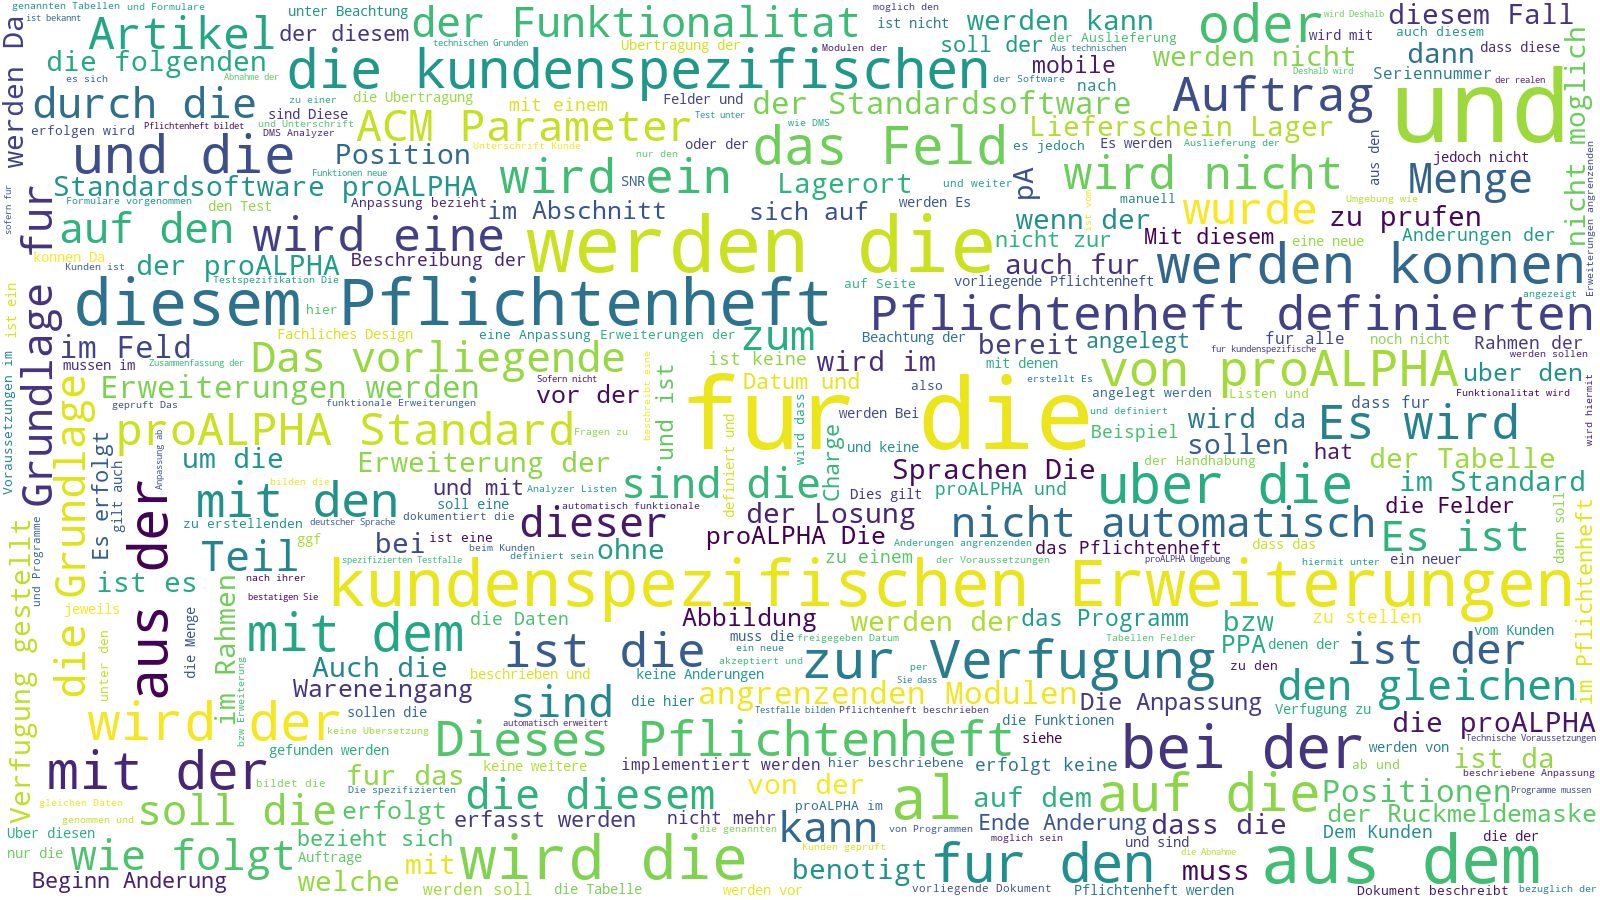
\includegraphics[width=6cm]{img/roh.png}
	\end{minipage}
	\hfill
	\begin{minipage}{0.48\textwidth}
		\centering
		\caption{Wordcloud 2 - nach Entfernung von deutschen \textit{stop-words}}
		\label{pic:wc-stops1}
		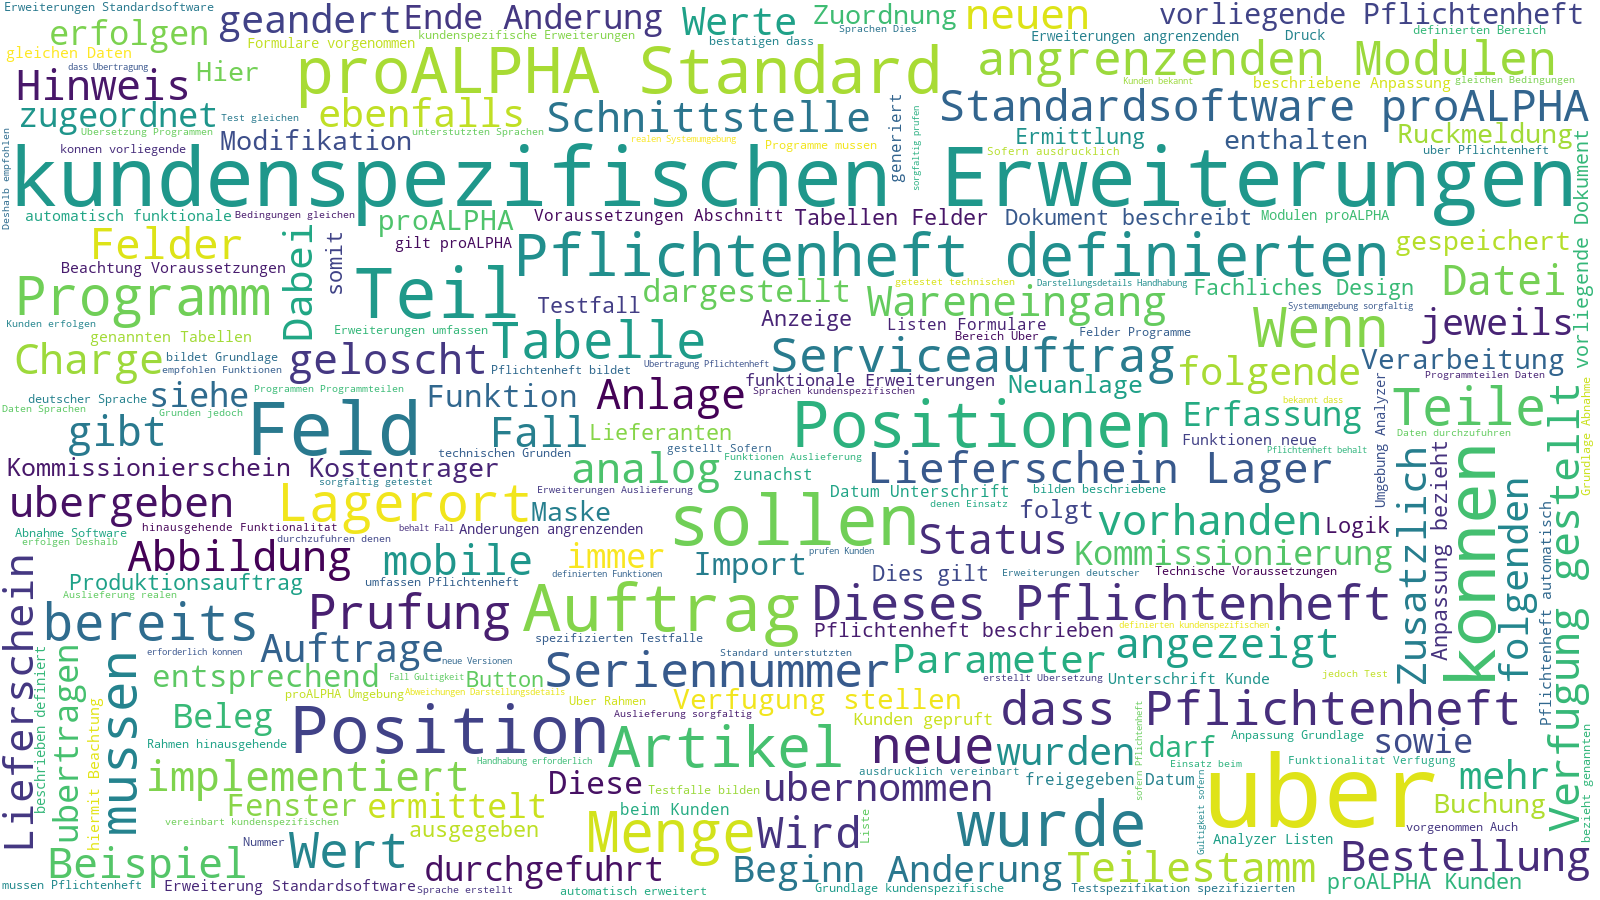
\includegraphics[width=6cm]{img/nurstop.png}		
	\end{minipage} 	
\end{figure}

\subsection{Unterabschnitt 1}

\begin{table}[htb]
	\centering
	\begin{tabular}{|c|c|c|c|} \hline
		Methode & \textit{Accuracy} & \textit{Precision} & \textit{Recall} \\ \hline
		hinge & 0.84541 & 0.83735 & 0.91285 \\
		log & 0.86956 & 0.83333 & 0.90452 \\
		modified\_huber & 0.86473 & 0.84278 & 0.91666 \\
		squared\_hinge & 0.69565 & 0.73129 & 0.78441 \\
		perceptron & \textbf{0.86956} & \textbf{0.85676} & \textbf{0.93871} \\ \hline
	\end{tabular}
	\caption{Durchschnittliche Performance für Durchlauf 1}
	\label{tab:methods-d1}
\end{table}

\blindtext{40}\\
\par
Hier verweise ich auf \ref{pic:wc-raw} und auf Abbildung \ref{pic:wc-stops1}\\
\par
\blindtext{60}


\pagebreak
\section{Fehlerbetrachtung}
\label{sec:fehler}

\blindtext{30}\par
\textcolor{red}{\textbf{Man sollte nicht außer Acht lassen, dass man das Bereits in der oen geziegten Tabelle \ref{tab:methods-d1} sieht.}}



	\chapter{Zusammenfassung und Ausblick}
\label{ch:conclusions}

\blindtext{30}

\section{Zusammenfassung der Ergebnisse}
\label{sec:conclusions}

\blindtext{250}

\section{Ausblick}
\label{sec:futurework}

\blindtext{150}

	\appendix
	%\include{related}
	%%\chapter{Anhänge}
\chapter{Detaillierte Ergebnisse und Daten}
\label{c:cs}
\unitlength1mm





	
%\cleardoublepage


%%%%%%%%%%%%%%%%%%%%%%%%%%%%%%%%%%%%%%%%%%%%%%%%%%%%%%%%%%%%%%%%%%%%%%%%%%%%%
%%% List of Todos
%%%%%%%%%%%%%%%%%%%%%%%%%%%%%%%%%%%%%%%%%%%%%%%%%%%%%%%%%%%%%%%%%%%%%%%%%%%%%



%%%%%%%%%%%%%%%%%%%%%%%%%%%%%%%%%%%%%%%%%%%%%%%%%%%%%%%%%%%%%%%%%%%%%%%%%%%%%
%%% Abkuerzungsverzeichnis
%%%%%%%%%%%%%%%%%%%%%%%%%%%%%%%%%%%%%%%%%%%%%%%%%%%%%%%%%%%%%%%%%%%%%%%%%%%%%

\chapter{Abkürzungen und Notationen}

%\chapter{Abkürzungsverzeichnis}
%\addcontentsline{toc}{section}{List of Abbreviations and Notations}

\subsubsection{Dataset and clustering acronyms}
\begin{table}[H]
	\begin{tabular}{cR{\textwidth}}
		\toprule
		Abkürzung & Bedeutung \\ \midrule
%A
%B
		\textbf{BoW} & Bag of Words \\
%C
%D
		\textbf{DTC} & Decision Tree Classifier \\
%E
%F
		\textbf{FN} & False Negatives \\
		\textbf{FP} & False Positives \\
%G
%H
%I
		\textbf{idf} & Inverse Document Frequency \\
%J
%K
%L
%M
%N
		\textbf{NB} & Naive Bayes \\
%O
%P
%Q
%R
		\textbf{RF} & Random Forest \\
%S
		\textbf{SVM} & Support Vector Machine \\
%T
		\textbf{tf} & Term Frequency \\
		\textbf{TN} & True Negatives \\
		\textbf{TP} & True Positives \\
%U
%V
%W
%X		
		$\mathbf{X}$ & Datensatz  \\
%Y
		$\mathbf{Y}$ & Resultat \\
%Z
		
		\bottomrule
	\end{tabular}	
\end{table}


\cleardoublepage

%%%%%%%%%%%%%%%%%%%%%%%%%%%%%%%%%%%%%%%%%%%%%%%%%%%%%%%%%%%%%%%%%%%%%%%%%%%%%
%%% Abbildungsverzeichnis
%%%%%%%%%%%%%%%%%%%%%%%%%%%%%%%%%%%%%%%%%%%%%%%%%%%%%%%%%%%%%%%%%%%%%%%%%%%%%

\chapter{Abbildungsverzeichnis}
\vspace{-0.3cm}
%\addcontentsline{toc}{section}{List of Figures}
\makeatletter
\@starttoc{lof}% Print List of Figures
\makeatother
\cleardoublepage

	
%%%%%%%%%%%%%%%%%%%%%%%%%%%%%%%%%%%%%%%%%%%%%%%%%%%%%%%%%%%%%%%%%%%%%%%%%%%%%
%%% Tabellenverzeichnis
%%%%%%%%%%%%%%%%%%%%%%%%%%%%%%%%%%%%%%%%%%%%%%%%%%%%%%%%%%%%%%%%%%%%%%%%%%%%%
	
\chapter{Tabellenverzeichnis}
\makeatletter
\@starttoc{lot}% Print List of Tables
\makeatother
\clearpage

%%%%%%%%%%%%%%%%%%%%%%%%%%%%%%%%%%%%%%%%%%%%%%%%%%%%%%%%%%%%%%%%%%%%%%%%%%%%%
%%% Algorithmenverzeichnis
%%%%%%%%%%%%%%%%%%%%%%%%%%%%%%%%%%%%%%%%%%%%%%%%%%%%%%%%%%%%%%%%%%%%%%%%%%%%%

\chapter{Verzeichnis der Algorithmen}
%\listofalgorithms
\begingroup
\renewcommand{\listalgorithmname}{}
\let\chapter\subsection% Make \chapter equivalent to \section
\listofalgorithms
\endgroup
%\makeatletter
%\@starttoc{loa}% Print List of Algorithms
%\makeatother
%%\listofalgorithms
	\chapter{Refrenzen}

\lipsum[5]


	%\include{index}

% =============================================================================
	\backmatter
	
	%\include{stmt}


\newpage
\thispagestyle{empty}
\begin{center}
	\vspace*{5em}
	\huge\textbf{Selbstständigkeitserklärung}\\
\end{center}
\vspace{2em}
Hiermit erkläre ich, die vorliegende Bachelorarbeit selbstständig, nur unter Zuhilfenahme der aufgeführten Quellen und Hilfsmittel, verfasst zu haben.

Die Arbeit wurde weder einer anderen Prüfungsbehörde vorgelegt noch veröffentlicht.

\vspace{4em}
\begin{minipage}{\linewidth}
	\begin{tabular}{p{15em}p{15em}}
		Datum: &  .......................................................\\
		& \centering (Unterschrift)\\
	\end{tabular}
\end{minipage}

\end{document}

         
